% Uncomment this to make slides with overlays:
%\documentclass[slides]{beamer}

% Uncomment these (but comment the above \documentclass line) to make handouts:
\documentclass[handout]{beamer}

% Uncomment these to have more than one slide per page
%\usepackage{pgfpages}
%\pgfpagesuselayout{2 on 1}[border shrink=5mm]
%\pgfpageslogicalpageoptions{1}{border code=\pgfusepath{stroke}}
%\pgfpageslogicalpageoptions{2}{border code=\pgfusepath{stroke}}

\usepackage[]{graphicx, color, hyperref}

\mode<presentation>
{
	%\usetheme[secheader]{Boadilla}
	%\usecolortheme[rgb={.835, .102,.169}]{structure}  
	\usetheme[width= 0cm]{Goettingen}
	%\setbeamercovered{transparent}
}
\setbeamertemplate{navigation symbols}{}
\setbeamertemplate{footline}[frame number]

\definecolor{blue2}{rgb}{0.278,0.278,0.729} 
\newcommand{\blue}[1]{\textcolor{blue2}{#1}}
\newcommand{\white}[1]{\textcolor{white}{#1}}
\newcommand{\red}[1]{\textcolor{red}{#1}}
\newcommand{\xbar}{\overline{x}}
\newcommand{\ybar}{\overline{y}}
\newcommand{\phat}{\widehat{p}}
\newcommand{\prob}{\mbox{Pr}}
\newcommand{\E}{\mathbb{E}}
\newcommand{\Var}{\mbox{Var}}
\newcommand{\cp}{\oplus}
\newcommand{\cm}{\circleddash}

\title{Lecture 5: Visualizing Numerical Data}
\author{Chapter 1.6 + 1.7}
\date{}

\begin{document}
%------------------------------------------------------------------------------
\begin{frame}
\titlepage
\end{frame}
%------------------------------------------------------------------------------



%------------------------------------------------------------------------------
\begin{frame}
\frametitle{Goals for Today}

\begin{itemize}
\item Visualizing numerical data
\begin{itemize}
\item Two famous historical examples of data visualization
\item Reed's 2013 entering class
\end{itemize}
\item Histograms
\item Measures of Central Tendency: Mean, Median, and Mode
\item Measure of Spread:  Sample variance and sample standard deviation
\end{itemize}

\end{frame}
%------------------------------------------------------------------------------


%------------------------------------------------------------------------------
\begin{frame}
\frametitle{Famous Example 1:  Napoleon's March on Russia in 1812}

In 1812, Napoleon led a French invasion of Russia, at one point marching on Moscow.  
\begin{center}
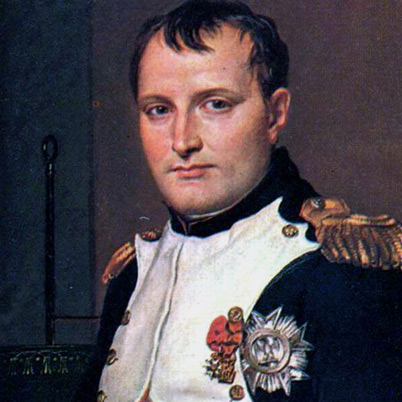
\includegraphics[height=0.6\textheight]{figure/napoleon.jpg}
\end{center}

\end{frame}
%------------------------------------------------------------------------------


%------------------------------------------------------------------------------
\begin{frame}
\frametitle{Famous Example 1:  Napoleon's March on Russia in 1812}

The advance and retreat on Moscow was an unmitigated disaster:
\begin{center}
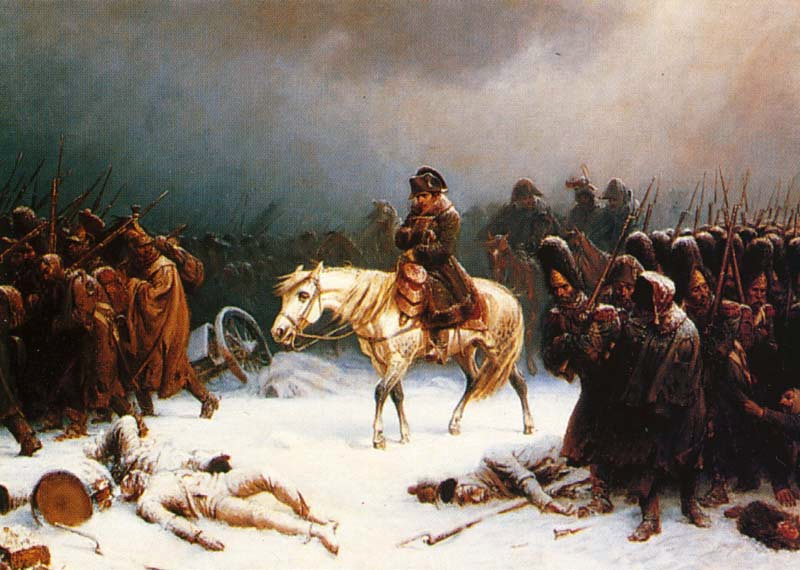
\includegraphics[height=0.6\textheight]{figure/retreat.jpg}
\end{center}


\end{frame}
%------------------------------------------------------------------------------



%------------------------------------------------------------------------------
\begin{frame}
\frametitle{Famous Example 1:  Napoleon's March on Russia in 1812}

\begin{center}
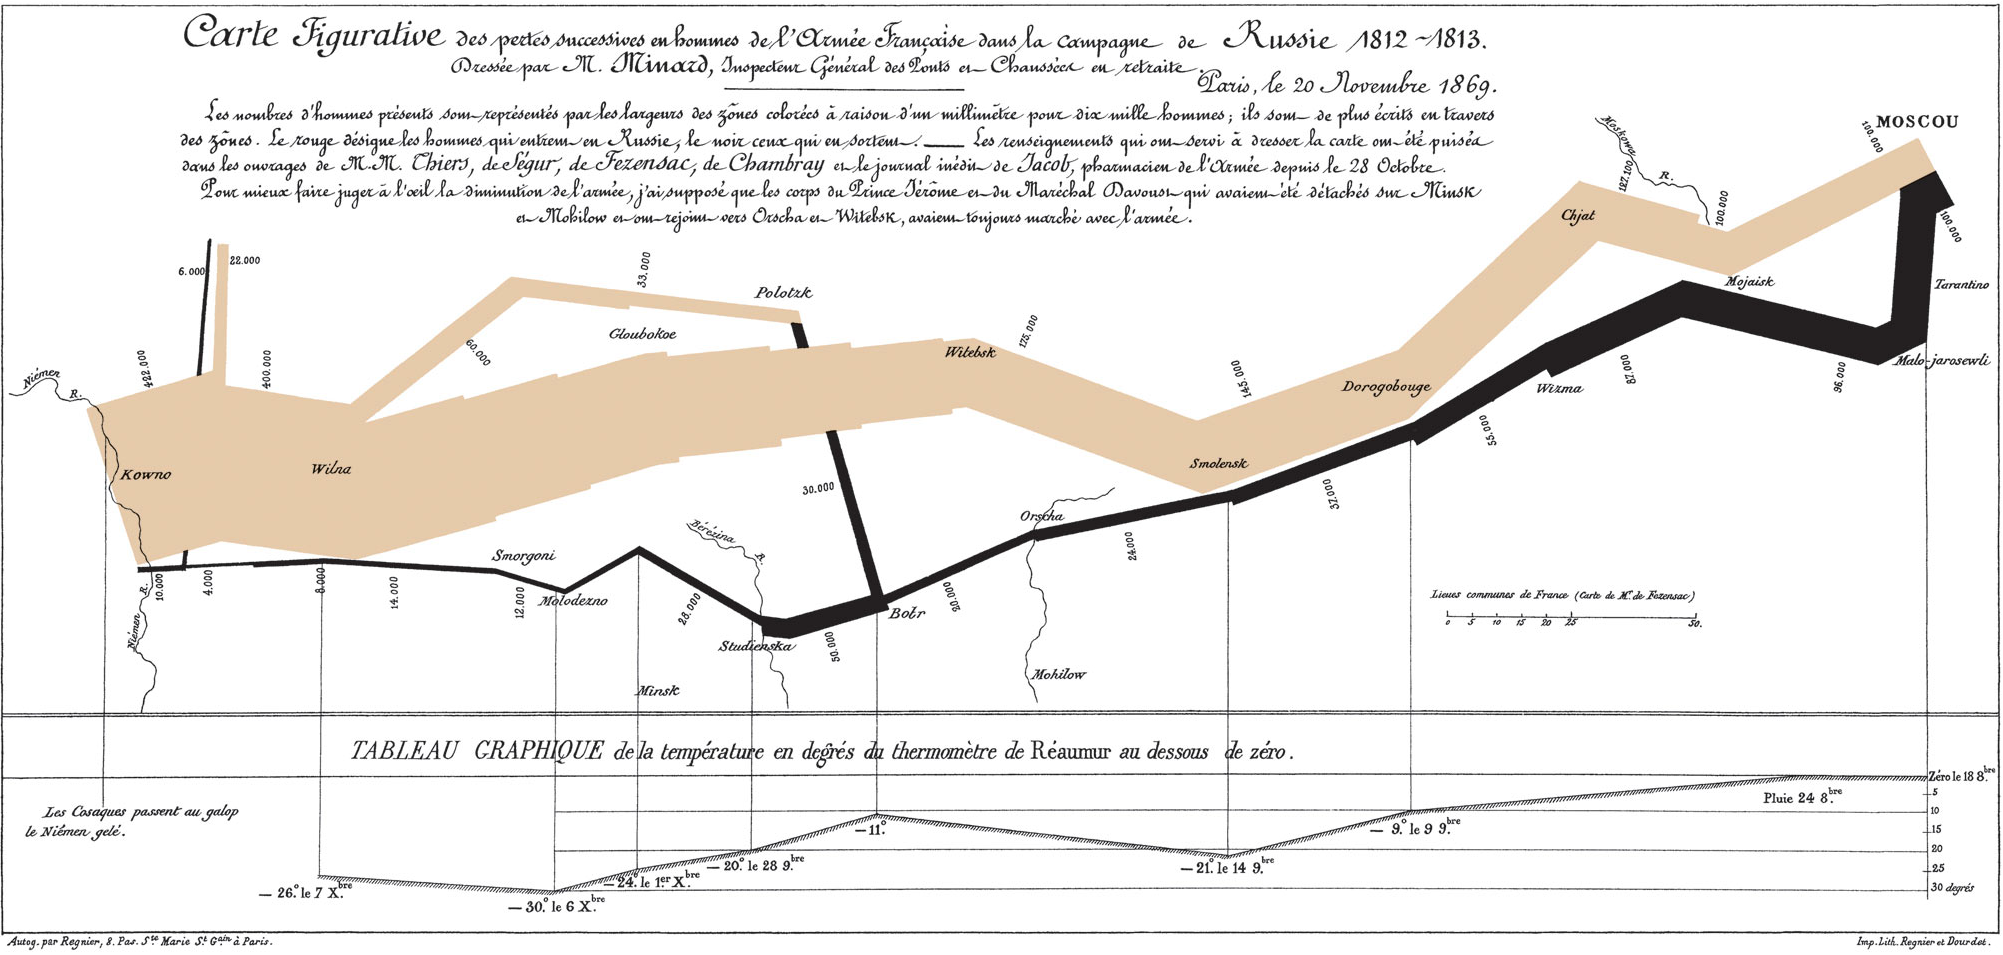
\includegraphics[width=\textwidth]{figure/Minard.png}
\end{center}

\end{frame}
%------------------------------------------------------------------------------



%------------------------------------------------------------------------------
\begin{frame}
\frametitle{Famous Example 1:  Napolean's March on Russia in 1812}
Why is this visualization big deal?

\vspace{0.5cm}

On a two-dimensional page, it displays 6 variables (in others words, 6 \blue{dimensions} of information) at once:
%\begin{enumerate}
%\pause \item Size of the army (width of bars)
%\pause \item Latitude
%\pause \item Longitude
%\pause \item Direction of the army:  advance (brown) or retreat (black)
%\pause \item Date
%\pause \item Temperature (on the bottom)
%\end{enumerate}

\vspace{5cm}

\end{frame}
%------------------------------------------------------------------------------


%------------------------------------------------------------------------------
\begin{frame}
\frametitle{Famous Example 2:  1854 Broad Street Cholera Outbreak}

On August 31 1854, an epidemic of cholera began in the Soho neighborhood of London.  Over the next three days 127 people near Broad Street had died.

\vspace{0.25cm}

\pause Dr. John Snow, a physician, was a student of the disease.  (From Wikipedia) Snow was a skeptic of the then-dominant \blue{miasma theory} that stated that diseases such as cholera or the Black Death were caused by pollution or a noxious form of ``bad air.'' 

\vspace{0.25cm}

\pause Snow created the following map to investigate:

\end{frame}
%------------------------------------------------------------------------------



%------------------------------------------------------------------------------
\begin{frame}
\frametitle{Famous Example 2:  1854 Broad Street Cholera Outbreak}

\begin{center}
\includegraphics[height=0.8\textheight]{figure/cholera1.png}
\end{center}

\end{frame}
%------------------------------------------------------------------------------


%------------------------------------------------------------------------------
\begin{frame}
\frametitle{Famous Example 2:  1854 Broad Street Cholera Outbreak}

\begin{center}
\includegraphics[height=0.8\textheight]{figure/cholera2.png}
\end{center}

\end{frame}
%------------------------------------------------------------------------------


%------------------------------------------------------------------------------
\begin{frame}
\frametitle{Famous Example 2:  1854 Broad Street Cholera Outbreak}

He identified the source of the outbreak as water from the \blue{Broad Street Pump}, which was near a cesspit that began to leak. 

\begin{center}
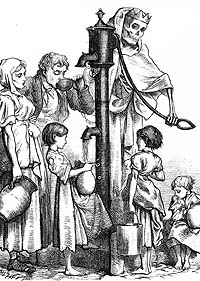
\includegraphics[height=4cm]{figure/king_cholera.jpg}
\end{center}

\pause This led to discovering that cholera was transmitted by food and water being contaminated by fecal matter and not via the air.  This was a watershed moment in the emerging field of \blue{epidemiology}.  

\end{frame}
%------------------------------------------------------------------------------


%------------------------------------------------------------------------------
\begin{frame}[fragile]
\frametitle{Histograms}
In the {\tt openintro} package, the {\tt email50} dataset contains a random sample of 50 emails, in which researchers try to identify emails as spam.  One variable is the \# of characters:

\vspace{0.25cm}

\begin{tiny}
\begin{verbatim}
Characters |  0-5  5-10  10-15  15-20  20-25  25-30  30-35  35-40  40-45  ...  60-65
(in 1000's)|
-------------------------------------------------------------------------------------------
Count      |   19    12      6      2      3      5      0      0      2  ...      1
\end{verbatim}
\end{tiny}

\vspace{0.25cm}

\pause So each of the intervals 0-5, 5-10, 10-15, etc. are \blue{buckets/bins} and we count the number of emails in each bucket/bin.  

\end{frame}
%------------------------------------------------------------------------------



%------------------------------------------------------------------------------
\begin{frame}[fragile]
\frametitle{Histograms}

Histograms provide a description of the shape of the \blue{distribution} of data.  

\begin{center}
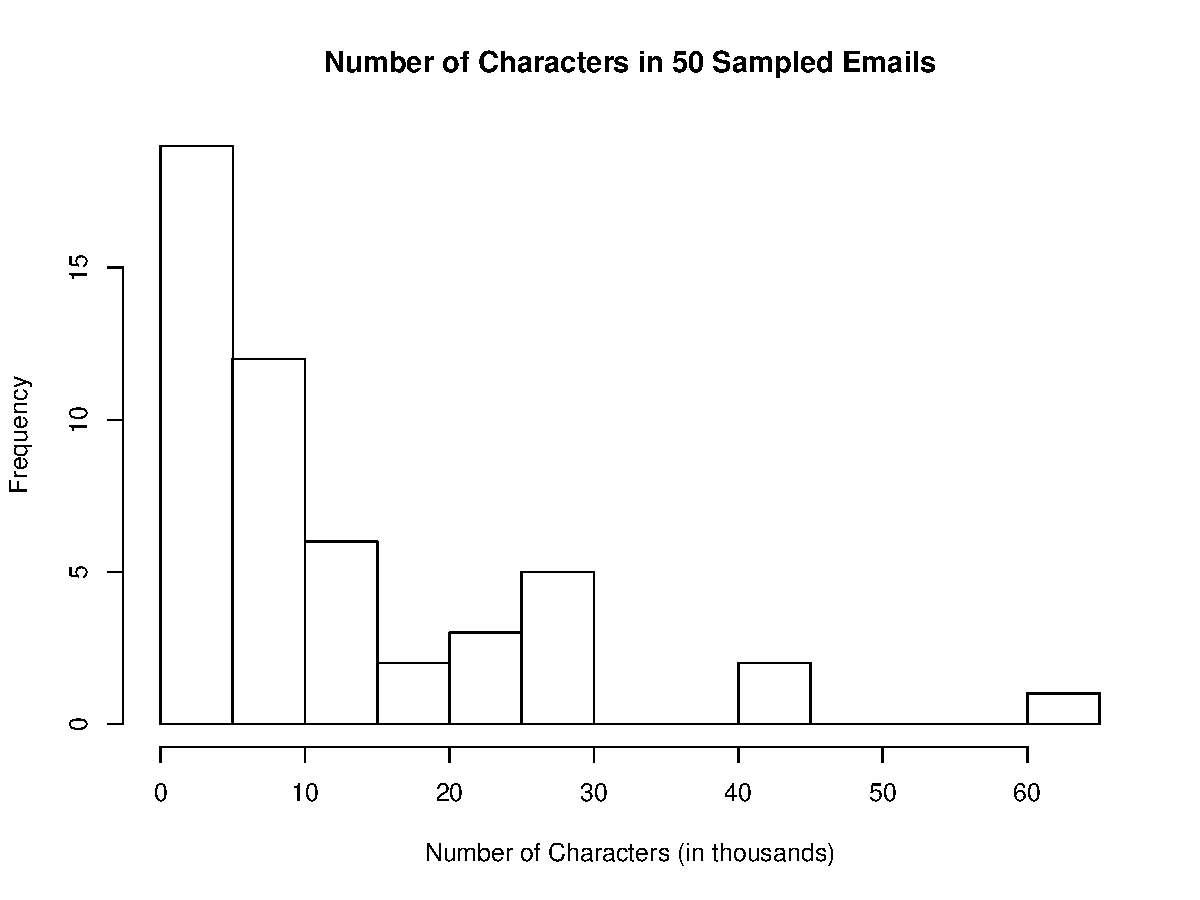
\includegraphics[height=0.7\textheight]{figure/hist.pdf}
\end{center}

\end{frame}
%------------------------------------------------------------------------------



%------------------------------------------------------------------------------
\begin{frame}[fragile]
\frametitle{Skew and Long Tail}
Also in the {\tt openintro} package is MLB salary data in 2010.  If we plot a histogram:

\begin{center}
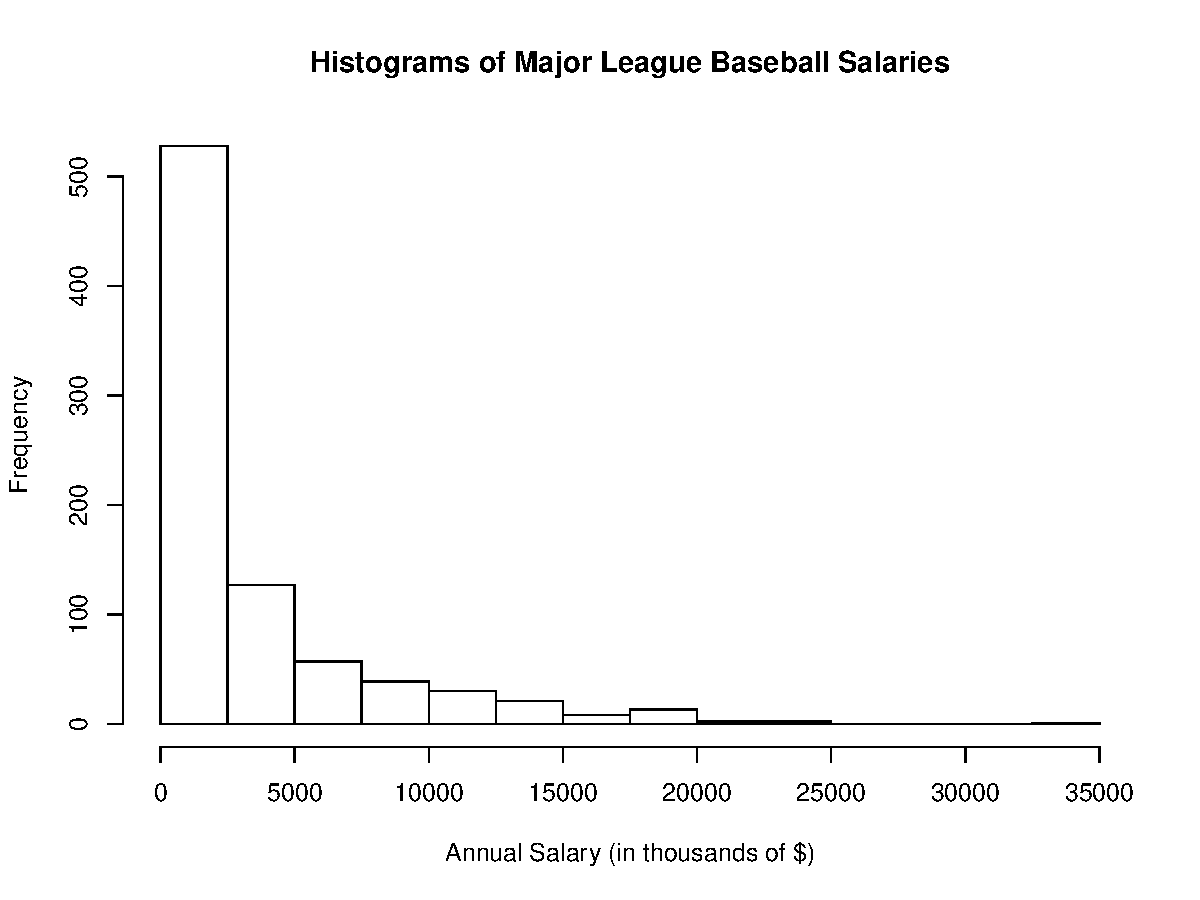
\includegraphics[height=5.5cm]{figure/MLB.pdf}
\end{center}

\pause The data has a \blue{long tail} to the right: data is \blue{right-skewed}.  i.e. a small number of players who make a VERY large amount of money.  

\end{frame}
%------------------------------------------------------------------------------



%------------------------------------------------------------------------------
\begin{frame}[fragile]
\frametitle{Trick to Remembering Which Skew is Which}

\begin{itemize}
\pause\item Long tail to the right: data is \blue{right-skewed} AKA \blue{positively-skewed}
\pause\item Long tail to the left: data is \blue{left-skewed} AKA \blue{negatively-skewed}
\end{itemize}

\begin{center}
\pause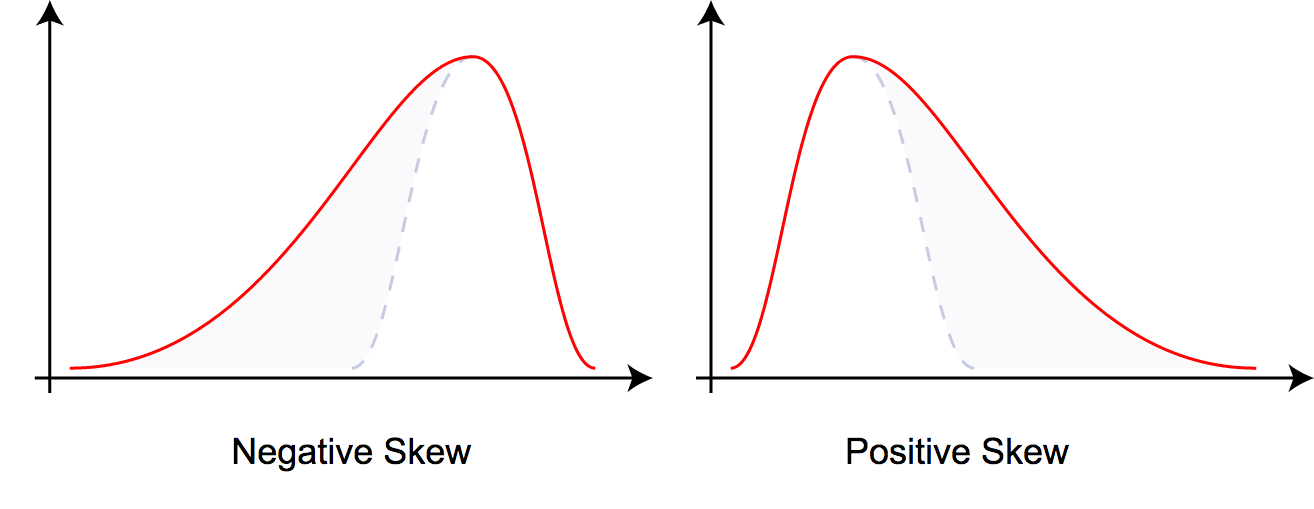
\includegraphics[width=10cm]{figure/skew.png}
\end{center}


\end{frame}
%------------------------------------------------------------------------------



%------------------------------------------------------------------------------
\begin{frame}
\frametitle{Reed's 2013 US-Originating Entering Class}
What can we do about skewed data?  

\vspace{1cm}

\blue{\url{http://rpubs.com/rudeboybert/reed2013}}

\end{frame}
%------------------------------------------------------------------------------


%------------------------------------------------------------------------------
\begin{frame}[fragile]
\frametitle{Mean}
The mean, AKA average, is a common way to measure the \blue{center} of the data.  So for example, the mean of 1, 2, 5, 3, and 7 is 
\[\frac{1 + 2 + 5 + 3 + 7}{5} = 3.6\]

\pause We label the \blue{sample mean} $\overline{x}$ (pronounced ``x bar''):
\[
\overline{x} = \frac{x_1 + x_2 + \ldots + x_n}{n}
\]
where $x_1, x_2, \ldots, x_n$ are the $n$ observed values.  
\end{frame}
%------------------------------------------------------------------------------


%------------------------------------------------------------------------------
\begin{frame}[fragile]
\frametitle{Median}
The \blue{median}, however, is the \blue{middle number}.

\vspace{0.5cm}

\pause Two cases:
\begin{itemize}
\item Odd number of values: the median of (1, 3, \blue{5}, 8, 10) is 5.
\item Even number of values: the median of (1, \blue{3, 5}, 8) is the average of the middle two values: $\frac{3+5}{2} = 4$
\end{itemize}

\vspace{0.5cm}

\pause But why use the median at all?

\end{frame}
%------------------------------------------------------------------------------


%-------------------------------------------------------------------------------
\begin{frame}
\frametitle{Mean vs Median: Imaginary Scenario}


\begin{itemize}
\item Say at company $X$, there 5 employees:  the CEO and everyone else.  
\pause\item The CEO earns \$1000 an hour, while the others earn \$20, \$21, \$30, and \$40 an hour. 
\pause\item The employees complain that they are paid too little.  
\pause\item The CEO counters that the mean hourly salary is $\overline{x}=\frac{20+21+30+40+1000}{5} = 222.20$ an hour, which is really high.
\end{itemize}

\end{frame}
%-------------------------------------------------------------------------------


%-------------------------------------------------------------------------------
\begin{frame}
\frametitle{Mean vs Median: Imaginary Scenario}
The CEO's extreme salary is inflating the mean.  A more appropriate measure is the median hourly salary of $30$.

\vspace{0.5cm}

\pause Medians are less sensitive to (i.e. more \blue{robust} to) \blue{outliers} than the mean.

\vspace{0.5cm}

\pause Ex: the ``median home price'' is typically used, because it isn't as sensitive as the mean to the few very expensive houses.
\end{frame}
%-------------------------------------------------------------------------------


%-------------------------------------------------------------------------------
\begin{frame}
\frametitle{Mean vs Median: Back to MLB Salary Data}

\begin{center}
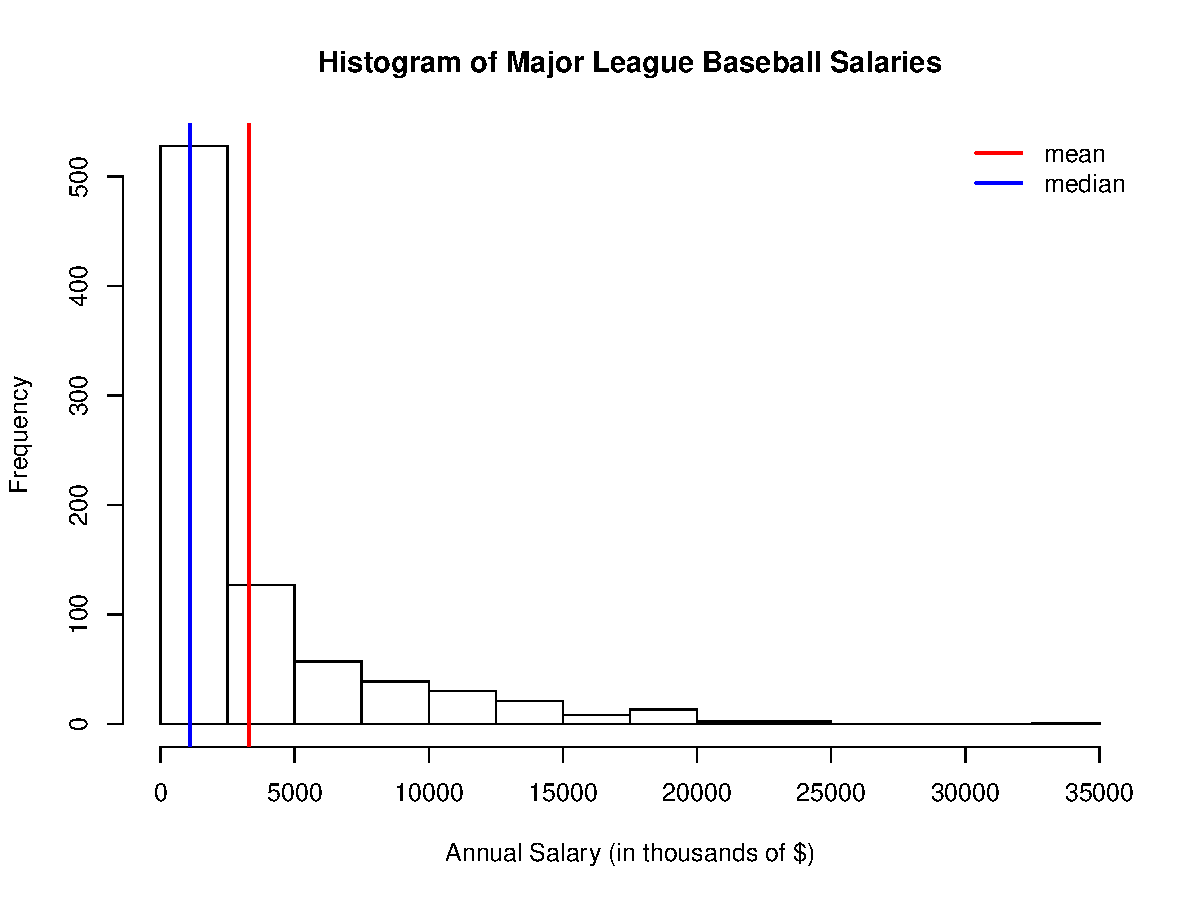
\includegraphics[height=5.5cm]{figure/MLB2.pdf}
\end{center}

\end{frame}
%-------------------------------------------------------------------------------


%------------------------------------------------------------------------------
\begin{frame}[fragile]
\frametitle{Mode}
A \blue{mode} is the value that appears the most often in a data set.  So out of (1, 3, 3, 5, 6), the modal value is 3.  

\vspace{0.25cm}

\pause Modes also describe \blue{peaks}, but this can get subjective. 

\vspace{0.25cm}

\pause A distribution can be \blue{unimodal}, \blue{bimodal}, or \blue{multimodal}:

\begin{center}
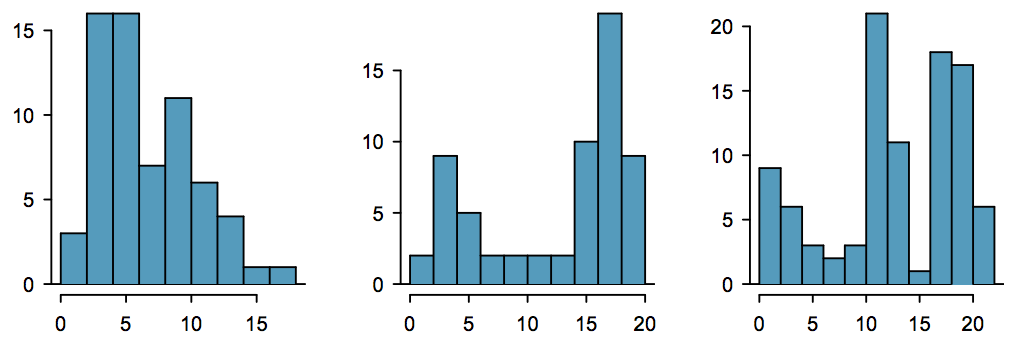
\includegraphics[height=3cm]{figure/modes.png}
\end{center}

\end{frame}
%------------------------------------------------------------------------------



%------------------------------------------------------------------------------
\begin{frame}[fragile]
\frametitle{Measure of Spread}

Next, consider the following two histograms:  Both have mean of about 20.  What is the difference between them?

\begin{center}
\pause 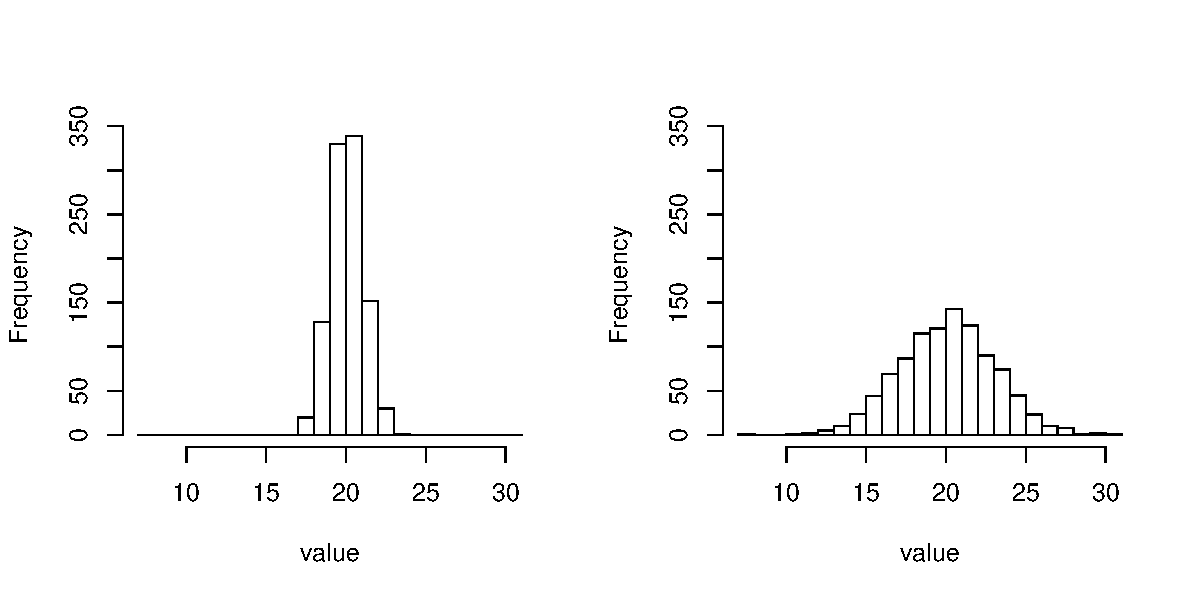
\includegraphics[width=\textwidth]{figure/spread.pdf}
\end{center}

\end{frame}
%------------------------------------------------------------------------------


%------------------------------------------------------------------------------
\begin{frame}[fragile]
\frametitle{Measure of Spread}

We need a measure of \blue{spread/variability}.  The \blue{sample variance $s^2$} is roughly the average squared distance from the mean.

\vspace{0.5cm}

The \blue{sample standard deviation $s$} is the square root of the sample variance. The sample standard deviation is useful when considering how close the data are to the mean.

\end{frame}
%------------------------------------------------------------------------------



%------------------------------------------------------------------------------
\begin{frame}[fragile]
\frametitle{Measure of Spread}
Back to example:
\begin{center}
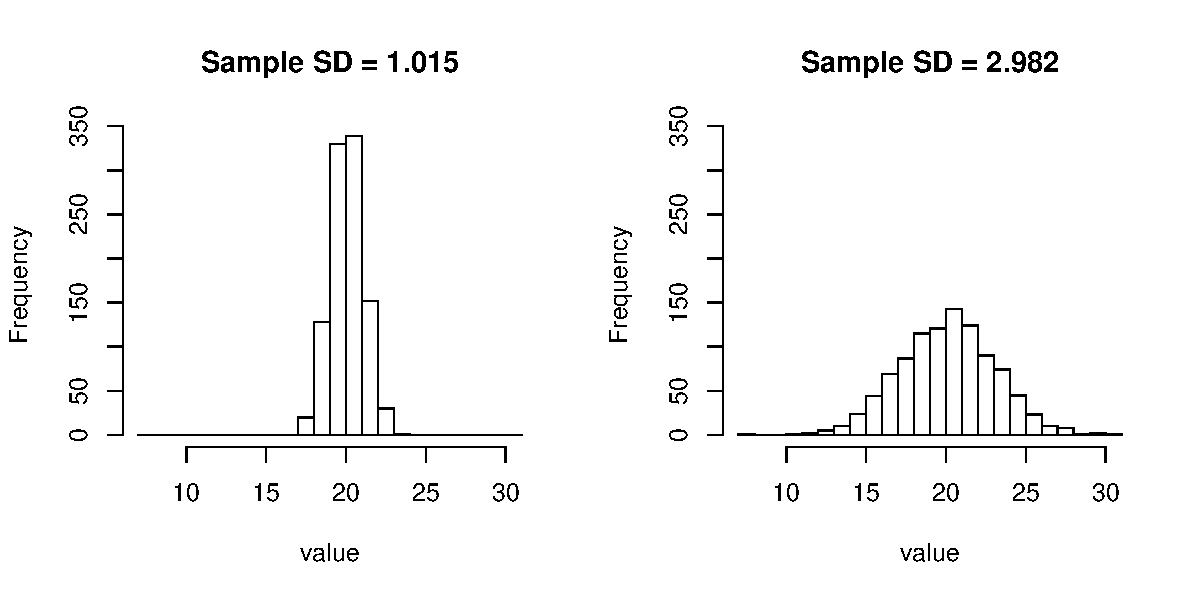
\includegraphics[width=\textwidth]{figure/spread2.pdf}
\end{center}

\end{frame}
%------------------------------------------------------------------------------



%------------------------------------------------------------------------------
\begin{frame}[fragile]
\frametitle{How to Compute the Sample Standard Deviation}

Read section 1.6.4.  The formula really doesn't make much intuitive sense, but is the way it is due to mathematical convenience.  Fortunately there is an {\tt R} command that computes it for you: {\tt sd()}

\end{frame}
%------------------------------------------------------------------------------



%------------------------------------------------------------------------------
\begin{frame}[fragile]
\frametitle{Next Time}

\begin{itemize}
\item Another simple data visualization tool: boxplots
\item Examining/Visualizing \blue{Categorical} Data
\end{itemize}


\end{frame}
%------------------------------------------------------------------------------







\end{document}










